
%% bare_conf.tex
%% V1.3
%% 2007/01/11
%% by Michael Shell
%% See:
%% http://www.michaelshell.org/
%% for current contact information.
%%
%% This is a skeleton file demonstrating the use of IEEEtran.cls
%% (requires IEEEtran.cls version 1.7 or later) with an IEEE conference paper.
%%
%% Support sites:
%% http://www.michaelshell.org/tex/ieeetran/
%% http://www.ctan.org/tex-archive/macros/latex/contrib/IEEEtran/
%% and
%% http://www.ieee.org/

%%*************************************************************************
%% Legal Notice:
%% This code is offered as-is without any warranty either expressed or
%% implied; without even the implied warranty of MERCHANTABILITY or
%% FITNESS FOR A PARTICULAR PURPOSE! 
%% User assumes all risk.
%% In no event shall IEEE or any contributor to this code be liable for
%% any damages or losses, including, but not limited to, incidental,
%% consequential, or any other damages, resulting from the use or misuse
%% of any information contained here.
%%
%% All comments are the opinions of their respective authors and are not
%% necessarily endorsed by the IEEE.
%%
%% This work is distributed under the LaTeX Project Public License (LPPL)
%% ( http://www.latex-project.org/ ) version 1.3, and may be freely used,
%% distributed and modified. A copy of the LPPL, version 1.3, is included
%% in the base LaTeX documentation of all distributions of LaTeX released
%% 2003/12/01 or later.
%% Retain all contribution notices and credits.
%% ** Modified files should be clearly indicated as such, including  **
%% ** renaming them and changing author support contact information. **
%%
%% File list of work: IEEEtran.cls, IEEEtran_HOWTO.pdf, bare_adv.tex,
%%                    bare_conf.tex, bare_jrnl.tex, bare_jrnl_compsoc.tex
%%*************************************************************************

% *** Authors should verify (and, if needed, correct) their LaTeX system  ***
% *** with the testflow diagnostic prior to trusting their LaTeX platform ***
% *** with production work. IEEE's font choices can trigger bugs that do  ***
% *** not appear when using other class files.                            ***
% The testflow support page is at:
% http://www.michaelshell.org/tex/testflow/



% Note that the a4paper option is mainly intended so that authors in
% countries using A4 can easily print to A4 and see how their papers will
% look in print - the typesetting of the document will not typically be
% affected with changes in paper size (but the bottom and side margins will).
% Use the testflow package mentioned above to verify correct handling of
% both paper sizes by the user's LaTeX system.
%
% Also note that the "draftcls" or "draftclsnofoot", not "draft", option
% should be used if it is desired that the figures are to be displayed in
% draft mode.
%
\documentclass[conference]{IEEEtran}
% Add the compsoc option for Computer Society conferences.
%
% If IEEEtran.cls has not been installed into the LaTeX system files,
% manually specify the path to it like:
% \documentclass[conference]{../sty/IEEEtran}



% Some very useful LaTeX packages include:
% (uncomment the ones you want to load)


% *** MISC UTILITY PACKAGES ***
%
%\usepackage{ifpdf}
% Heiko Oberdiek's ifpdf.sty is very useful if you need conditional
% compilation based on whether the output is pdf or dvi.
% usage:
% \ifpdf
%   % pdf code
% \else
%   % dvi code
% \fi
% The latest version of ifpdf.sty can be obtained from:
% http://www.ctan.org/tex-archive/macros/latex/contrib/oberdiek/
% Also, note that IEEEtran.cls V1.7 and later provides a builtin
% \ifCLASSINFOpdf conditional that works the same way.
% When switching from latex to pdflatex and vice-versa, the compiler may
% have to be run twice to clear warning/error messages.






% *** CITATION PACKAGES ***
%
%\usepackage{cite}
% cite.sty was written by Donald Arseneau
% V1.6 and later of IEEEtran pre-defines the format of the cite.sty package
% \cite{} output to follow that of IEEE. Loading the cite package will
% result in citation numbers being automatically sorted and properly
% "compressed/ranged". e.g., [1], [9], [2], [7], [5], [6] without using
% cite.sty will become [1], [2], [5]--[7], [9] using cite.sty. cite.sty's
% \cite will automatically add leading space, if needed. Use cite.sty's
% noadjust option (cite.sty V3.8 and later) if you want to turn this off.
% cite.sty is already installed on most LaTeX systems. Be sure and use
% version 4.0 (2003-05-27) and later if using hyperref.sty. cite.sty does
% not currently provide for hyperlinked citations.
% The latest version can be obtained at:
% http://www.ctan.org/tex-archive/macros/latex/contrib/cite/
% The documentation is contained in the cite.sty file itself.






% *** GRAPHICS RELATED PACKAGES ***
%
%  \usepackage{subfigure}
\ifCLASSINFOpdf
   \usepackage[pdftex]{graphicx}
  % declare the path(s) where your graphic files are
  % \graphicspath{{../pdf/}{../jpeg/}}
  % and their extensions so you won't have to specify these with
  % every instance of \includegraphics
  % \DeclareGraphicsExtensions{.pdf,.jpeg,.png}
\else
  % or other class option (dvipsone, dvipdf, if not using dvips). graphicx
  % will default to the driver specified in the system graphics.cfg if no
  % driver is specified.
  \usepackage[dvips]{graphicx}
  % declare the path(s) where your graphic files are
  % \graphicspath{{../eps/}}
  % and their extensions so you won't have to specify these with
  % every instance of \includegraphics
  % \DeclareGraphicsExtensions{.eps}
\fi
% graphicx was written by David Carlisle and Sebastian Rahtz. It is
% required if you want graphics, photos, etc. graphicx.sty is already
% installed on most LaTeX systems. The latest version and documentation can
% be obtained at: 
% http://www.ctan.org/tex-archive/macros/latex/required/graphics/
% Another good source of documentation is "Using Imported Graphics in
% LaTeX2e" by Keith Reckdahl which can be found as epslatex.ps or
% epslatex.pdf at: http://www.ctan.org/tex-archive/info/
%
% latex, and pdflatex in dvi mode, support graphics in encapsulated
% postscript (.eps) format. pdflatex in pdf mode supports graphics
% in .pdf, .jpeg, .png and .mps (metapost) formats. Users should ensure
% that all non-photo figures use a vector format (.eps, .pdf, .mps) and
% not a bitmapped formats (.jpeg, .png). IEEE frowns on bitmapped formats
% which can result in "jaggedy"/blurry rendering of lines and letters as
% well as large increases in file sizes.
%
% You can find documentation about the pdfTeX application at:
% http://www.tug.org/applications/pdftex





% *** MATH PACKAGES ***
%
%\usepackage[cmex10]{amsmath}
% A popular package from the American Mathematical Society that provides
% many useful and powerful commands for dealing with mathematics. If using
% it, be sure to load this package with the cmex10 option to ensure that
% only type 1 fonts will utilized at all point sizes. Without this option,
% it is possible that some math symbols, particularly those within
% footnotes, will be rendered in bitmap form which will result in a
% document that can not be IEEE Xplore compliant!
%
% Also, note that the amsmath package sets \interdisplaylinepenalty to 10000
% thus preventing page breaks from occurring within multiline equations. Use:
%\interdisplaylinepenalty=2500
% after loading amsmath to restore such page breaks as IEEEtran.cls normally
% does. amsmath.sty is already installed on most LaTeX systems. The latest
% version and documentation can be obtained at:
% http://www.ctan.org/tex-archive/macros/latex/required/amslatex/math/





% *** SPECIALIZED LIST PACKAGES ***
%
%\usepackage{algorithmic}
% algorithmic.sty was written by Peter Williams and Rogerio Brito.
% This package provides an algorithmic environment fo describing algorithms.
% You can use the algorithmic environment in-text or within a figure
% environment to provide for a floating algorithm. Do NOT use the algorithm
% floating environment provided by algorithm.sty (by the same authors) or
% algorithm2e.sty (by Christophe Fiorio) as IEEE does not use dedicated
% algorithm float types and packages that provide these will not provide
% correct IEEE style captions. The latest version and documentation of
% algorithmic.sty can be obtained at:
% http://www.ctan.org/tex-archive/macros/latex/contrib/algorithms/
% There is also a support site at:
% http://algorithms.berlios.de/index.html
% Also of interest may be the (relatively newer and more customizable)
% algorithmicx.sty package by Szasz Janos:
% http://www.ctan.org/tex-archive/macros/latex/contrib/algorithmicx/




% *** ALIGNMENT PACKAGES ***
%
%\usepackage{array}
% Frank Mittelbach's and David Carlisle's array.sty patches and improves
% the standard LaTeX2e array and tabular environments to provide better
% appearance and additional user controls. As the default LaTeX2e table
% generation code is lacking to the point of almost being broken with
% respect to the quality of the end results, all users are strongly
% advised to use an enhanced (at the very least that provided by array.sty)
% set of table tools. array.sty is already installed on most systems. The
% latest version and documentation can be obtained at:
% http://www.ctan.org/tex-archive/macros/latex/required/tools/


%\usepackage{mdwmath}
%\usepackage{mdwtab}
% Also highly recommended is Mark Wooding's extremely powerful MDW tools,
% especially mdwmath.sty and mdwtab.sty which are used to format equations
% and tables, respectively. The MDWtools set is already installed on most
% LaTeX systems. The lastest version and documentation is available at:
% http://www.ctan.org/tex-archive/macros/latex/contrib/mdwtools/


% IEEEtran contains the IEEEeqnarray family of commands that can be used to
% generate multiline equations as well as matrices, tables, etc., of high
% quality.


%\usepackage{eqparbox}
% Also of notable interest is Scott Pakin's eqparbox package for creating
% (automatically sized) equal width boxes - aka "natural width parboxes".
% Available at:
% http://www.ctan.org/tex-archive/macros/latex/contrib/eqparbox/





% *** SUBFIGURE PACKAGES ***
%\usepackage[tight,footnotesize]{subfigure}
% subfigure.sty was written by Steven Douglas Cochran. This package makes it
% easy to put subfigures in your figures. e.g., "Figure 1a and 1b". For IEEE
% work, it is a good idea to load it with the tight package option to reduce
% the amount of white space around the subfigures. subfigure.sty is already
% installed on most LaTeX systems. The latest version and documentation can
% be obtained at:
% http://www.ctan.org/tex-archive/obsolete/macros/latex/contrib/subfigure/
% subfigure.sty has been superceeded by subfig.sty.



%\usepackage[caption=false]{caption}
%\usepackage[font=footnotesize]{subfig}
% subfig.sty, also written by Steven Douglas Cochran, is the modern
% replacement for subfigure.sty. However, subfig.sty requires and
% automatically loads Axel Sommerfeldt's caption.sty which will override
% IEEEtran.cls handling of captions and this will result in nonIEEE style
% figure/table captions. To prevent this problem, be sure and preload
% caption.sty with its "caption=false" package option. This is will preserve
% IEEEtran.cls handing of captions. Version 1.3 (2005/06/28) and later 
% (recommended due to many improvements over 1.2) of subfig.sty supports
% the caption=false option directly:
%\usepackage[caption=false,font=footnotesize]{subfig}
%
% The latest version and documentation can be obtained at:
% http://www.ctan.org/tex-archive/macros/latex/contrib/subfig/
% The latest version and documentation of caption.sty can be obtained at:
% http://www.ctan.org/tex-archive/macros/latex/contrib/caption/




% *** FLOAT PACKAGES ***
%
%\usepackage{fixltx2e}
% fixltx2e, the successor to the earlier fix2col.sty, was written by
% Frank Mittelbach and David Carlisle. This package corrects a few problems
% in the LaTeX2e kernel, the most notable of which is that in current
% LaTeX2e releases, the ordering of single and double column floats is not
% guaranteed to be preserved. Thus, an unpatched LaTeX2e can allow a
% single column figure to be placed prior to an earlier double column
% figure. The latest version and documentation can be found at:
% http://www.ctan.org/tex-archive/macros/latex/base/



%\usepackage{stfloats}
% stfloats.sty was written by Sigitas Tolusis. This package gives LaTeX2e
% the ability to do double column floats at the bottom of the page as well
% as the top. (e.g., "\begin{figure*}[!b]" is not normally possible in
% LaTeX2e). It also provides a command:
%\fnbelowfloat
% to enable the placement of footnotes below bottom floats (the standard
% LaTeX2e kernel puts them above bottom floats). This is an invasive package
% which rewrites many portions of the LaTeX2e float routines. It may not work
% with other packages that modify the LaTeX2e float routines. The latest
% version and documentation can be obtained at:
% http://www.ctan.org/tex-archive/macros/latex/contrib/sttools/
% Documentation is contained in the stfloats.sty comments as well as in the
% presfull.pdf file. Do not use the stfloats baselinefloat ability as IEEE
% does not allow \baselineskip to stretch. Authors submitting work to the
% IEEE should note that IEEE rarely uses double column equations and
% that authors should try to avoid such use. Do not be tempted to use the
% cuted.sty or midfloat.sty packages (also by Sigitas Tolusis) as IEEE does
% not format its papers in such ways.





% *** PDF, URL AND HYPERLINK PACKAGES ***
%
%\usepackage{url}
% url.sty was written by Donald Arseneau. It provides better support for
% handling and breaking URLs. url.sty is already installed on most LaTeX
% systems. The latest version can be obtained at:
% http://www.ctan.org/tex-archive/macros/latex/contrib/misc/
% Read the url.sty source comments for usage information. Basically,
% \url{my_url_here}.


% \usepackage[colorinlistoftodos,textsize=small,backgroundcolor=yellow]{todonotes}
\usepackage{url}


% *** Do not adjust lengths that control margins, column widths, etc. ***
% *** Do not use packages that alter fonts (such as pslatex).         ***
% There should be no need to do such things with IEEEtran.cls V1.6 and later.
% (Unless specifically asked to do so by the journal or conference you plan
% to submit to, of course. )


% correct bad hyphenation here
\hyphenation{op-tical net-works semi-conduc-tor}


\begin{document}

\title{SkyscrapAR: Visualizing Software \\ Evolution with Augmented Reality}


% author names and affiliations
% use a multiple column layout for up to three different
% affiliations

% \author{
% \IEEEauthorblockN{Rodrigo Souza, Bruno Silva, Thiago Mendes, Manoel Mendon\c{c}a}
% \IEEEauthorblockA{Software Engineering Lab, Computer Science Department\\
% Federal University of Bahia, Bahia, Brazil\\
% Email: \{rodrigo, brunocs, thiagomendes, mgmendonca\}@dcc.ufba.br}
% }

\author{
	\IEEEauthorblockN{
		Rodrigo Souza\IEEEauthorrefmark{1},
		Bruno Silva\IEEEauthorrefmark{1},
		Thiago Mendes\IEEEauthorrefmark{1}\IEEEauthorrefmark{2} and 
		Manoel Mendon\c{c}a\IEEEauthorrefmark{1}\IEEEauthorrefmark{3}
	}

	\IEEEauthorblockA{
		\IEEEauthorrefmark{1}
		Software Engineering Lab, Computer Science Department\\
		Federal University of Bahia, Bahia, Brazil \\
		Email: \{rodrigo, brunocs\}@dcc.ufba.br
	}

	\IEEEauthorblockA{
		\IEEEauthorrefmark{2}
		Information Technology Department, Federal Institute of Bahia\\
		Campus Santo Amaro, Bahia, Brazil \\
		Email: thiagomendes@dcc.ufba.br
	}

	\IEEEauthorblockA{
		\IEEEauthorrefmark{3}
		Fraunhofer Project Center on Software and System Engineering\\
		Federal University of Bahia, Bahia, Brazil \\
		Email: mgmendonca@dcc.ufba.br
	}
}



% conference papers do not typically use \thanks and this command
% is locked out in conference mode. If really needed, such as for
% the acknowledgment of grants, issue a \IEEEoverridecommandlockouts
% after \documentclass

% for over three affiliations, or if they all won't fit within the width
% of the page, use this alternative format:
% 
%\author{\IEEEauthorblockN{Michael Shell\IEEEauthorrefmark{1},
%Homer Simpson\IEEEauthorrefmark{2},
%James Kirk\IEEEauthorrefmark{3}, 
%Montgomery Scott\IEEEauthorrefmark{3} and
%Eldon Tyrell\IEEEauthorrefmark{4}}
%\IEEEauthorblockA{\IEEEauthorrefmark{1}School of Electrical and Computer Engineering\\
%Georgia Institute of Technology,
%Atlanta, Georgia 30332--0250\\ Email: see http://www.michaelshell.org/contact.html}
%\IEEEauthorblockA{\IEEEauthorrefmark{2}Twentieth Century Fox, Springfield, USA\\
%Email: homer@thesimpsons.com}
%\IEEEauthorblockA{\IEEEauthorrefmark{3}Starfleet Academy, San Francisco, California 96678-2391\\
%Telephone: (800) 555--1212, Fax: (888) 555--1212}
%\IEEEauthorblockA{\IEEEauthorrefmark{4}Tyrell Inc., 123 Replicant Street, Los Angeles, California 90210--4321}}




% use for special paper notices
%\IEEEspecialpapernotice{(Invited Paper)}




% make the title area
\maketitle


\begin{abstract}
  Many authors have proposed three-dimensional visualizations to assist in the understanding and development of software. However, it is not natural to navigate through such visualizations using keyboard and mouse, and equipment such as virtual reality gloves and glasses are too expensive. In this paper we present SkyscrapAR, an augmented reality visualization that uses the city metaphor to represent the evolution of the software, along with its potential applications in practice. The use of augmented reality allows the user to interact with the city in an intuitive way by manipulating a marker printed on a paper. The hardware requirements are minimal: just a computer with a camera. Such features make SkyscrapAR a good fit for design reviews either within the workplace or in a videoconference setting. 
Video demonstration at http://youtu.be/... \todo{URL}

Keywords�  3D software visualization; augmented reality; software evolution

\end{abstract}
% IEEEtran.cls defaults to using nonbold math in the Abstract.
% This preserves the distinction between vectors and scalars. However,
% if the conference you are submitting to favors bold math in the abstract,
% then you can use LaTeX's standard command \boldmath at the very start
% of the abstract to achieve this. Many IEEE journals/conferences frown on
% math in the abstract anyway.

% no keywords




% For peer review papers, you can put extra information on the cover
% page as needed:
% \ifCLASSOPTIONpeerreview
% \begin{center} \bfseries EDICS Category: 3-BBND \end{center}
% \fi
%
% For peerreview papers, this IEEEtran command inserts a page break and
% creates the second title. It will be ignored for other modes.
\IEEEpeerreviewmaketitle


\section{Introduction} \label{sec:intro}
Software systems evolve by nature \cite{lehman:1980}. The activity of software development becomes more complex as the system evolves, which leads to the need for preventive and corrective maintenance. This complexity is reflected in the fact that about 90\% of the total costs of software systems are associated with their maintenance \cite{erlikh:2000}. Therefore, the area represents a promising field for improvement.

Visualization techniques have been used in software engineering as a possible solution to the difficult task of understanding, maintaining and evolving software systems. The visual metaphors are very useful in this context because sight is the most developed sense in human being \cite{diehl:2007}.

During the last decade, tools such as CodeCity~\cite{wettel:2008} have used 3D visualizations to represent, and hopefully provide a better understanding of, software. 3D visualization is sometimes more intuitive and has an extra dimension that allows the visualization of a larger amounts of information in relation to 2D visualization \cite{teyseyre:2009}. However, it also has an important limitation. The computer screen is bi-dimensional and always occludes something that is represented three dimensionally. A solution to the problem of interaction between the user and 3D software is the use of augmented reality. This technology makes virtual objects visible in real environments, facilitating virtual interaction with the user, since the communication can be done through gestures and movements \cite{azuma:1997}.

This paper presents SkyscrapAR, a new software evolution visualization approach that uses a city metaphor combined with augmented reality techniques. SkyscrapAR represents software classes and packages as 3D buildings of a chosen project revision number. These buildings are laid over on a terrain baseline blueprint derived from all versions of the software project. Buildings are sized up and colored by their size and number of changes. The project revision displayed can be dynamically chosen and buildings can be dynamically filtered for better evolution analysis. The augmented reality approach allows for easy manipulation of the produced visual scenarios. To the best of our knowledge, there is no other work in the literature that uses this approach.

This paper is structured as follows. Section 2 presents SkyscrapAR and its features. Then, Section 3 discusses some applications of the tool. Finally, Section 4 concludes this article.

\section{SkyscrapAR} \label{sec:skyscrapar}
SkyscrapAR is an augmented reality (AR) software evolution visualization based on the metaphor of an evolving city. Similarly to CodeCity~\cite{wettel:2008}, SkyscrapAR represents packages (or folders in the source code file structure) as rectangular city lots, with sub-packages being stacked on top of the package containing them (see Figure~\ref{fig:sample_junit}). Classes (or source code implementation files) are represented by buildings (boxes with different areas and heights) located on top of their respective packages, with the area they occupy being proportional to the size of the class, measured in lines of code. The user can browse over revisions of the software, and see buildings appearing, disappearing, and changing their shape to reflect successive modifications that they suffered over time.

\begin{figure}[ht!]
 \centering
 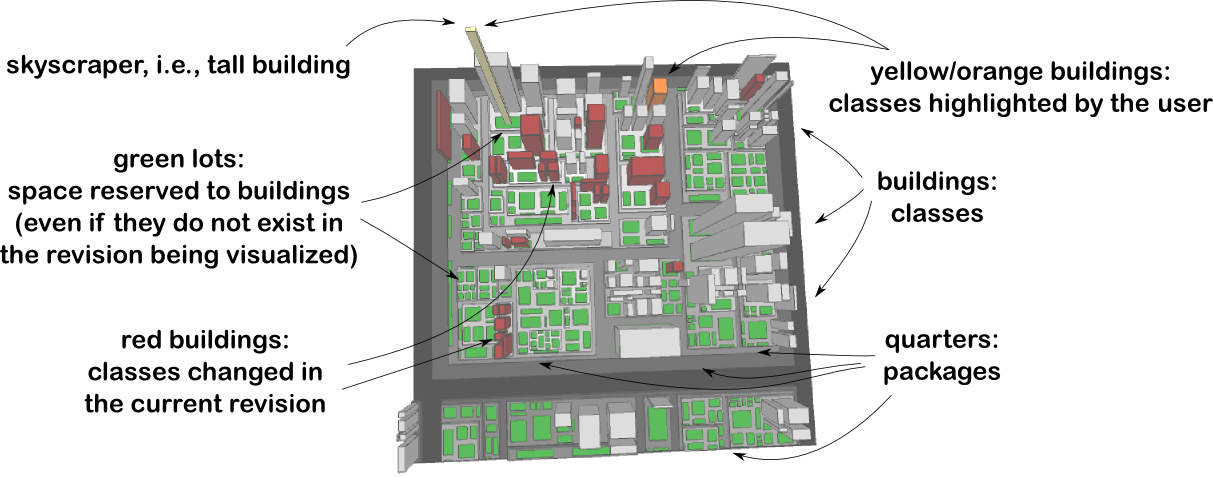
\includegraphics[width=0.5\textwidth, bb=0 0 1214 477]{./images/infographic}
 % fig1 - infographic.png: 1213x477 pixel, 72dpi, 42.82x16.84 cm, bb=0 0 1214 477
 \caption{The JUnit framework visualized as a city using SkyscrapAR.}
 \label{fig:sample_junit}
\end{figure}

Because the city (i.e., the software) evolves over time, it must have space to accommodate all buildings that existed in some period of its history. That is why the city terrain is divided in green lots, each one belonging to a building (i.e., a class). Green lots are large enough to fit their respective buildings when they reach maximum area. So, for example, buildings which present some green area in the last revision represent classes that used to be larger but had their size reduced.

The full source code is also publicly available under an open source license\footnote{\url{https://github.com/rodrigorgs/SkyscrapAR}}. The rest of this section describes SkyscrapAR in terms of its architecture, used source code metrics, and its user interface.

\subsection{Architecture} \label{sec:architecture}
SkyscrapAR is composed of two executables: the extractor and the viewer. The extractor, written in Java, reads a local Git repository containing Java source code and outputs a XML file describing its revisions, along with information for each source code file that was modified in each revision. The viewer, written in Processing\footnote{\url{http://processing.org/}}, takes the XML file and presents its data as a city that the user can view and interact with.

\begin{figure}[ht!]
 \centering
 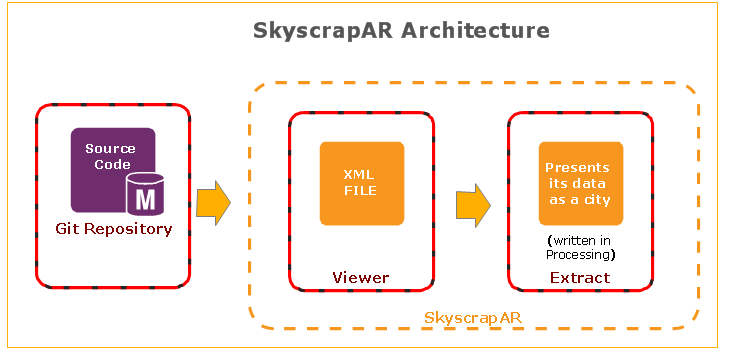
\includegraphics[width=0.5\textwidth, bb=0 0 547 269]{./images/architecture}
 % architecture.png: 729x359 pixel, 96dpi, 19.29x9.50 cm, bb=0 0 547 269
 \caption{SkyscrapAR architecture}
 \label{fig:architecture}
\end{figure}

The hardware setup needed to use the visualization is printed marker and a computer with screen and camera, as shown in Figure~\ref{fig:setup}. A marker is a piece of paper or any other object with a predefined black and white square pattern printed on it. The marker signals where the city will be rendered appear within the user’s environment. The user interacts with the visualization as he would do with a mock-up city, manipulating the marker with the hands so the city can be seen from the desired viewpoint.

\begin{figure}[h!]
 \centering
 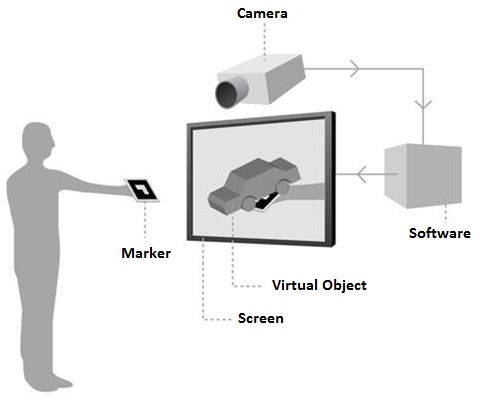
\includegraphics[width=0.4\textwidth, bb=0 0 486 406]{./images/howtowork.jpg}
 % howtowork.jpg: 479x400 pixel, 71dpi, 17.14x14.31 cm, bb=0 0 486 406
 \caption{Augmented reality setup.}
 \label{fig:setup}
\end{figure}

The processing needed for augmented reality is shown in Figure~\ref{fig:rendering_visualization}. Each frame captured by the camera is converted to a binary, black and white image, according to configurable brightness threshold. An algorithm then detects black square contours and then compares its inside with a predefined pattern. If they match, then it builds a local 3D coordinate system for the marker, as shown in Figure~\ref{fig:rendering_visualization}b. The 3D model of the city is then aligned with the local coordinate axes, as shown in Figure~\ref{fig:rendering_visualization}c, so it moves together with the marker, giving the effect that it is a part of the real world.

\begin{figure}[ht!]
 \centering
 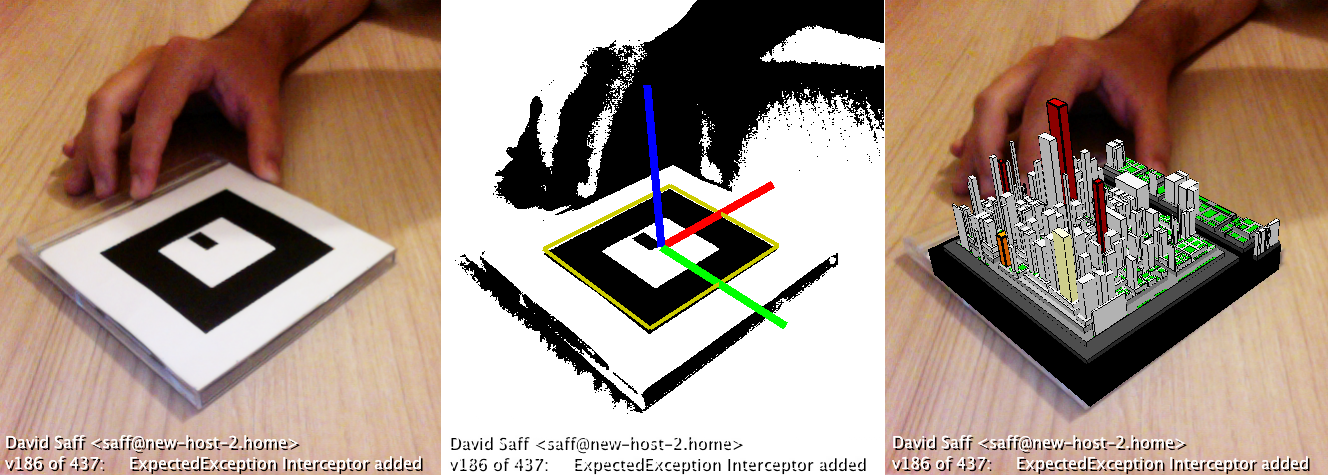
\includegraphics[width=0.5\textwidth, bb=14 14 1343 490]{./images/visualizationRedering}
 % visualizationRedering.eps: 0x0 pixel, 300dpi, 0.00x0.00 cm, bb=14 14 1343 490
 \caption{Rendering the visualization scene with augmented reality}
 \label{fig:rendering_visualization}
\end{figure}

\subsection{Mapping Metrics to Visual Elements} \label{sec:metrics_visual_elements}
A software system is composed of consecutive revisions. In each revision, two metrics are computed for all the classes: number of lines of code (LOC) and code churn. 

The LOC metric is the total number of lines in the respective source code file, including comments and blank lines. This metric, although simple to measure, correlates with many traditional complexity metrics that are used to predict development effort and fault proneness \cite{elemam:2001}.

Code churn refers to how much a particular file has been modified in its current and previous revisions in the version control system. The code churn of a class in its initial revision is equal to its LOC. Then, each time the class is modified, the code churn is incremented by the number of lines of code added or removed in the revision, as computed by Unix’s diff tool. That way, code churn always increases or is kept constant over time. The rationale for code churn is that source code files modified frequently are less stable and tend to be more prone to faults \cite{nagappan:2005}.

\subsection{User Interface} \label{sec:user_interface}
The user interface for SkyscrapAR displays the scene being captured by the camera and, if a marker is on the scene, the 3D model of the city is superimposed on it. In the bottom part of the screen, information about the current revision being visualized is displayed. It includes the sequential number of the revision, together with the name of the developer responsible for the change and the message describing the change.

Contrary to what happens in most 3D software visualizations, where users change their viewpoint by using the mouse or the keyboard, in SkyscrapAR, the user can view the city from different angles by manipulating either the 3D marker or the camera. With such interaction mechanism, the user can explore all six degrees of freedom of the 3D space (translation and rotation along three axes) in a natural way. For instance, the city can be seen from the top, in an aerial view, evidencing the structure of the software, or sideways, in a skyline view, evidencing skyscrapers, i.e., classes with high code churn.

In its current state, SkyscrapAR still depends on mouse and keyboard input, although we plan to reduce this dependency. The mouse pointer is used to highlight classes the user may want to focus on. The keyboard is mainly used to navigate through revisions, using the left and right arrow keys.

When the user advances the visualization to the next revision, buildings representing classes that were modified in that revision appear in red, so they can be easily spotted among the default gray buildings. It is expected that the buildings in red changed its shape compared to the previous revision 1 to reflect changes in the number of lines of code (area of the base) or in its code churn (height). Such changes in shape are presented as a smooth animation, by interpolating the dimensions of the buildings over a short period of time (less than one second). That way, it is easier to track the changes in the classes over time, enhancing the perception of evolution.

When the mouse pointer is over a building, the interface shows information for the respective class: name, package containing it, and the values for the LOC and code churn metrics. The user can also highlight a set of buildings, which get painted in yellow, by clicking on them. If a class is highlighted and has changed in the current revision, it gets painted in orange instead (i.e., a red and yellow mix). 

The purpose of the highlighting is twofold: it helps the user track the position of some buildings while exploring the visualization, and enables the user to focus on the changes of the highlighted buildings. When at least one building is selected, the navigation among revisions is restricted to revisions in which at least one highlighted class is changed. This is useful to study the evolution of a single class or of a set of classes.

By pressing the "H"� key on the keyboard, the user can switch between two view modes. In the default mode, all classes are shown. In the focused mode, only highlighted classes and classes changed in the current revision are shown. This mode helps the user to analyze the scattering of changes throughout the packages. When combined with the restricted navigation that takes place when classes are highlighted, it also enables the user to visualize classes that evolve together within a given set of classes.

\section{Applications in Software Development Practice} \label{sec:applications}

Researchers have found demand for agile assessments, that is, a kind of software product assessment that may provide valuable information rapidly and cheaply to support program understanding and maintenance \cite{nierstrasz:2012}. We envision several applications of SkycrapAR in this context. This section describes some of them and shows screenshots of the tool to illustrate typical situations (see Figure 3).

\begin{figure*}[t]
 \centering
 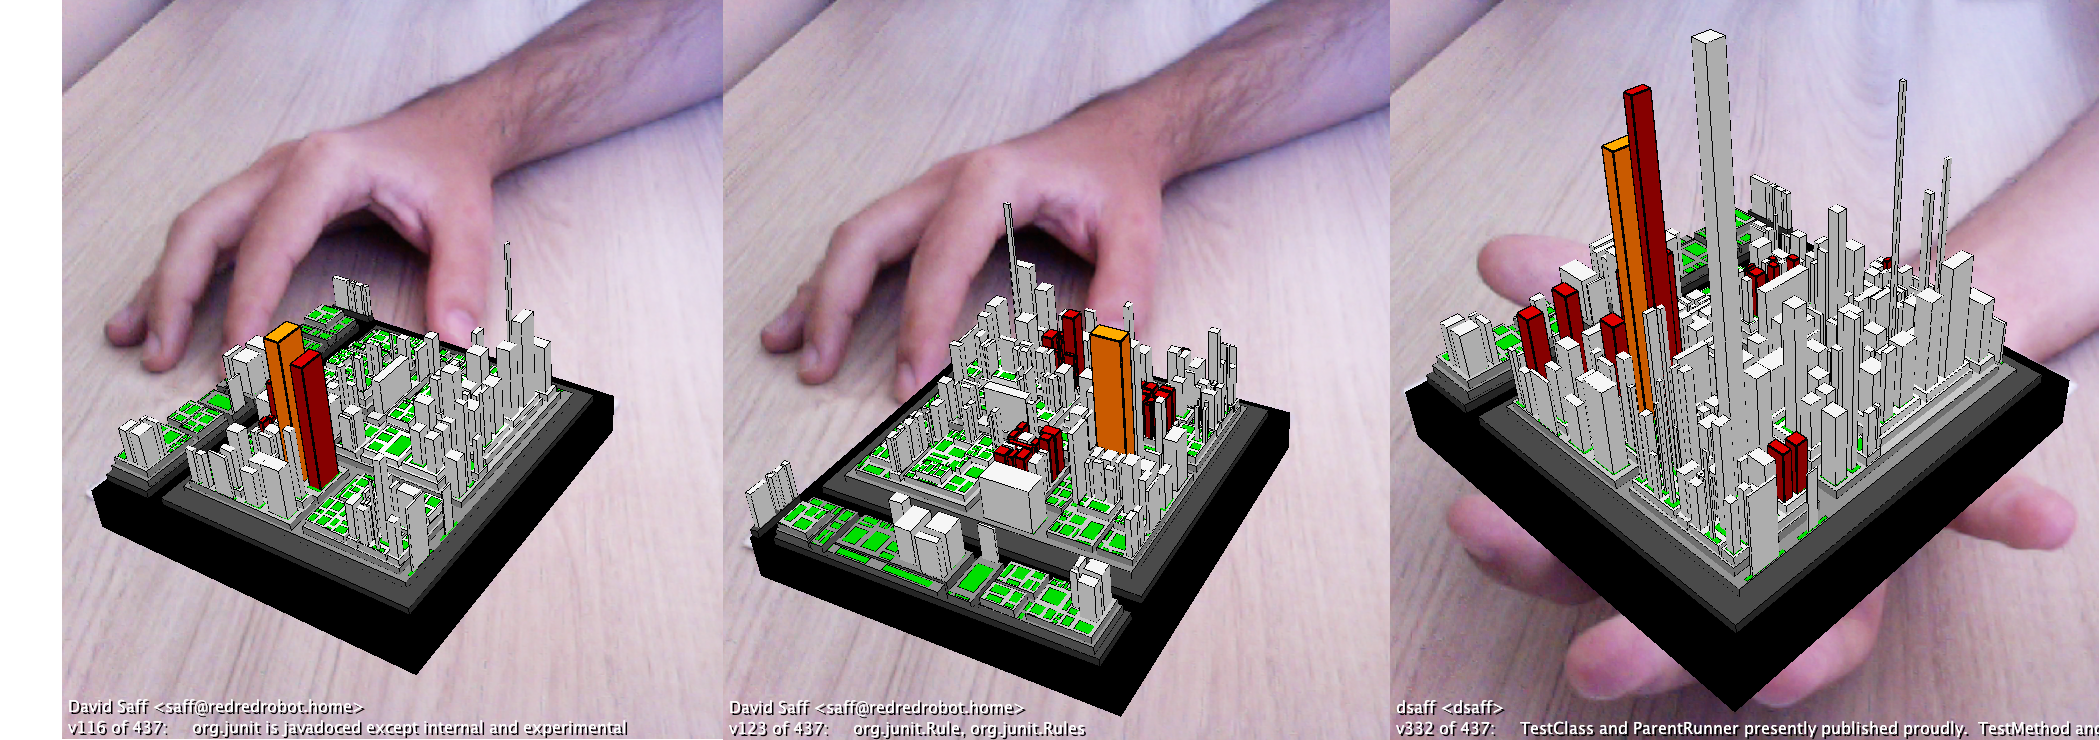
\includegraphics[width=0.8\textwidth, bb=14 14 2114 755]{./images/applications}
 % applications.eps: 0x0 pixel, 300dpi, 0.00x0.00 cm, bb=14 14 2114 755
 \caption{Three distinct versions of the JUnit framework in which the class BlockJUnit4ClassRunner (highlighted in orange) was modified.}
 \label{fig:TOBEDEFINED}
\end{figure*}

\textbf{Finding Skyscrapers.} In a software project, it is common to find classes which change a lot—the so called change-prone classes. In SkyscrapAR, they can be easily found as skyscrapers (see the orange building in Figure 3). Analog to the real concept, skyscrapers in our visualization are classes that concentrate a lot of the development effort. These classes deserve special attention, since they are more likely to be fault-prone \cite{nagappan:2005}. 

\textbf{Visualizing Scattering of Changes.} Source code management systems usually list packages and classes that were changed in each revision, but there is no visual information about the scattering of each commit transaction that generates a revision. This is easily done in SkycrapAR (see red buildings in Figure 3). Identifying scattered changes is important, as they represent modifications that impacted several systems modules, pointing out system-wide maintenance activities, such as refactoring’s or move operations among folders, or indicating that there are too many dependencies between software modules.

\textbf{Visualizing Classes Co-change.} Sometimes, classes have logical couplings even if they are not explicitly coupled to each other by their internal structural elements \cite{gall:1998}. Classes may be connected by means of implicit abstract elements related to the domain. For example, classes that are not structurally coupled but implement concerns that are strongly dependent at the requirements level. SkycrapAR provides information about the classes co-change by highlighting in red the classes that changed together in each revision (see Figure 3). 

\textbf{Finding God Classes.} A god class is a well-known code smell which refers to classes that perform too much work on its own. It breaks one of the basic principles of object-oriented design which states that a class should have one single responsibility. Also, implementing several responsibilities are more likely to undergo changes as much as the evolution history targets the responsibilities implemented by the class \cite{silva:2012}. SkyscrapAR helps developer to reason about god classes using the High Occupation of Territory metaphor - tall buildings occupying large areas.

\textbf{Identifying Populous Districts and City Centers.} Normally systems as cities have one or more neighborhoods with tall buildings and packages with no or very few green area - those areas are Populous Districts. This observation can be interpreted as the most touched parts of the system. If there is only a single well-defined populous district, we call it the City Center. Finding the city center (or other populous districts) may be useful to focus code inspection and testing on the most modified and possibly the most fault-prone parts of the system. It may also help to find refactoring opportunities on specific packages that suffered too many changes

\section{Final Remarks} \label{sec:finalRemarks}
This paper presented SkyscrapAR, an augmented reality visualization that employs the city metaphor to display information about the evolution of a software system. To the best of our knowledge, this is the first software visualization tool to employ augmented reality. In addition to describing SkyscrapAR, the paper shows how it can be used to support software comprehension tasks.

Currently, the tool has some limitations. In its current stage, only Java source code is supported, although it should be easy to add support for other languages. Also, it is limited to display one software system at a time, even if multiple markers are used. Finally, the user interaction still relies on the use of mouse and keyboard, which reduces the sense of immersion that characterizes augmented reality applications.

As future work, we intend to investigate interaction modes that dispense the use of mouse and keyboard. Our goal is to create a user interface that is intuitive, while discarding approaches that require expensive equipment such as virtual reality helmets and gloves. We also plan to make better use of colors in the visualization in order to display richer information. For instance, buildings can be painted in different colors to represent distinct crosscutting concerns implemented by them or, still, the developers who have contributed to the class. We plan to evaluate the tool with developers in academic or industrial settings. The evaluation should focus on usability and the effectiveness of the tool when used to support specific software comprehension tasks.

\section*{Acknowledgment}
The authors wish to thank Michele Lanza for encouraging this publication.


% \section{Introduction}
% % no \IEEEPARstart
% This demo file is intended to serve as a ``starter file''
% for IEEE conference papers produced under \LaTeX\ using
% IEEEtran.cls version 1.7 and later.
% % You must have at least 2 lines in the paragraph with the drop letter
% % (should never be an issue)
% I wish you the best of success.

% \hfill mds
 
% \hfill January 11, 2007

% \subsection{Subsection Heading Here}
% Subsection text here.


% \subsubsection{Subsubsection Heading Here}
% Subsubsection text here.


% % An example of a floating figure using the graphicx package.
% % Note that \label must occur AFTER (or within) \caption.
% % For figures, \caption should occur after the \includegraphics.
% % Note that IEEEtran v1.7 and later has special internal code that
% % is designed to preserve the operation of \label within \caption
% % even when the captionsoff option is in effect. However, because
% % of issues like this, it may be the safest practice to put all your
% % \label just after \caption rather than within \caption{}.
% %
% % Reminder: the "draftcls" or "draftclsnofoot", not "draft", class
% % option should be used if it is desired that the figures are to be
% % displayed while in draft mode.
% %
% %\begin{figure}[!t]
% %\centering
% %\includegraphics[width=2.5in]{myfigure}
% % where an .eps filename suffix will be assumed under latex, 
% % and a .pdf suffix will be assumed for pdflatex; or what has been declared
% % via \DeclareGraphicsExtensions.
% %\caption{Simulation Results}
% %\label{fig_sim}
% %\end{figure}

% % Note that IEEE typically puts floats only at the top, even when this
% % results in a large percentage of a column being occupied by floats.


% % An example of a double column floating figure using two subfigures.
% % (The subfig.sty package must be loaded for this to work.)
% % The subfigure \label commands are set within each subfloat command, the
% % \label for the overall figure must come after \caption.
% % \hfil must be used as a separator to get equal spacing.
% % The subfigure.sty package works much the same way, except \subfigure is
% % used instead of \subfloat.
% %
% %\begin{figure*}[!t]
% %\centerline{\subfloat[Case I]\includegraphics[width=2.5in]{subfigcase1}%
% %\label{fig_first_case}}
% %\hfil
% %\subfloat[Case II]{\includegraphics[width=2.5in]{subfigcase2}%
% %\label{fig_second_case}}}
% %\caption{Simulation results}
% %\label{fig_sim}
% %\end{figure*}
% %
% % Note that often IEEE papers with subfigures do not employ subfigure
% % captions (using the optional argument to \subfloat), but instead will
% % reference/describe all of them (a), (b), etc., within the main caption.


% % An example of a floating table. Note that, for IEEE style tables, the 
% % \caption command should come BEFORE the table. Table text will default to
% % \footnotesize as IEEE normally uses this smaller font for tables.
% % The \label must come after \caption as always.
% %
% %\begin{table}[!t]
% %% increase table row spacing, adjust to taste
% %\renewcommand{\arraystretch}{1.3}
% % if using array.sty, it might be a good idea to tweak the value of
% % \extrarowheight as needed to properly center the text within the cells
% %\caption{An Example of a Table}
% %\label{table_example}
% %\centering
% %% Some packages, such as MDW tools, offer better commands for making tables
% %% than the plain LaTeX2e tabular which is used here.
% %\begin{tabular}{|c||c|}
% %\hline
% %One & Two\\
% %\hline
% %Three & Four\\
% %\hline
% %\end{tabular}
% %\end{table}


% % Note that IEEE does not put floats in the very first column - or typically
% % anywhere on the first page for that matter. Also, in-text middle ("here")
% % positioning is not used. Most IEEE journals/conferences use top floats
% % exclusively. Note that, LaTeX2e, unlike IEEE journals/conferences, places
% % footnotes above bottom floats. This can be corrected via the \fnbelowfloat
% % command of the stfloats package.



% \section{Conclusion}
% The conclusion goes here.




% % conference papers do not normally have an appendix


% % use section* for acknowledgement
% \section*{Acknowledgment}


% The authors would like to thank...





% % trigger a \newpage just before the given reference
% % number - used to balance the columns on the last page
% % adjust value as needed - may need to be readjusted if
% % the document is modified later
% %\IEEEtriggeratref{8}
% % The "triggered" command can be changed if desired:
% %\IEEEtriggercmd{\enlargethispage{-5in}}

% % references section

% % can use a bibliography generated by BibTeX as a .bbl file
% % BibTeX documentation can be easily obtained at:
% % http://www.ctan.org/tex-archive/biblio/bibtex/contrib/doc/
% % The IEEEtran BibTeX style support page is at:
% % http://www.michaelshell.org/tex/ieeetran/bibtex/
% % argument is your BibTeX string definitions and bibliography database(s)
% %\bibliography{IEEEabrv,../bib/paper}
% %
% % <OR> manually copy in the resultant .bbl file
% % set second argument of \begin to the number of references
% % (used to reserve space for the reference number labels box)
% \begin{thebibliography}{1}

% \bibitem{IEEEhowto:kopka}
% H.~Kopka and P.~W. Daly, \emph{A Guide to \LaTeX}, 3rd~ed.\hskip 1em plus
%   0.5em minus 0.4em\relax Harlow, England: Addison-Wesley, 1999.

% \end{thebibliography}

\bibliographystyle{IEEEtran}
\bibliography{skyscrapar-icse2013}

% that's all folks
\end{document}


